\documentclass[12pt, a4paper]{article}
\usepackage{graphicx}

\title{Fish Sorting Minigame}

\begin{document}
\maketitle

\section{Overall Concept}
The player is given a trickle of fish that they need to sort based on habitat requirements. At the start of the game, this is as simple as whether the water is fresh water or salt water, but as the game goes on, difficulty ramps up by feeding fish to the player at a faster rate, or potentially by adding more habitats with more differences the player needs to account for, such as water temperature. The player starts with three lives and loses one for incorrectly sorting a fish or for letting a fish remain unsorted for too long. When the player runs out of lives, the game ends.

\subsection{Game Purpose}
The purpose of the game is to measure the player's ability to learn to differentiate between different fish species and memorize their habitat requirements. In order to perform well at the game, the player needs to be able to quickly absorb the habitat information it presents to them and memorize the needs of a dozen or so different fish, as they won't have time to check the info for each fish as the game speeds up. Performing well in this game would either indicate that the player is predisposed with knowledge about marine biology, or is able to efficiently adapt to new information.

\subsection{Controls}
The player can hover the mouse over a fish to receive the name of the fish as well as a list of habitat conditions it needs to survive. The player can click and hold a fish to grab it, but while grabbed no information is displayed about it. The player can then release the fish in one of the habitat categories, and is awarded a point if it is correctly placed.

\subsection{Presentation}
\begin{figure}
\centering
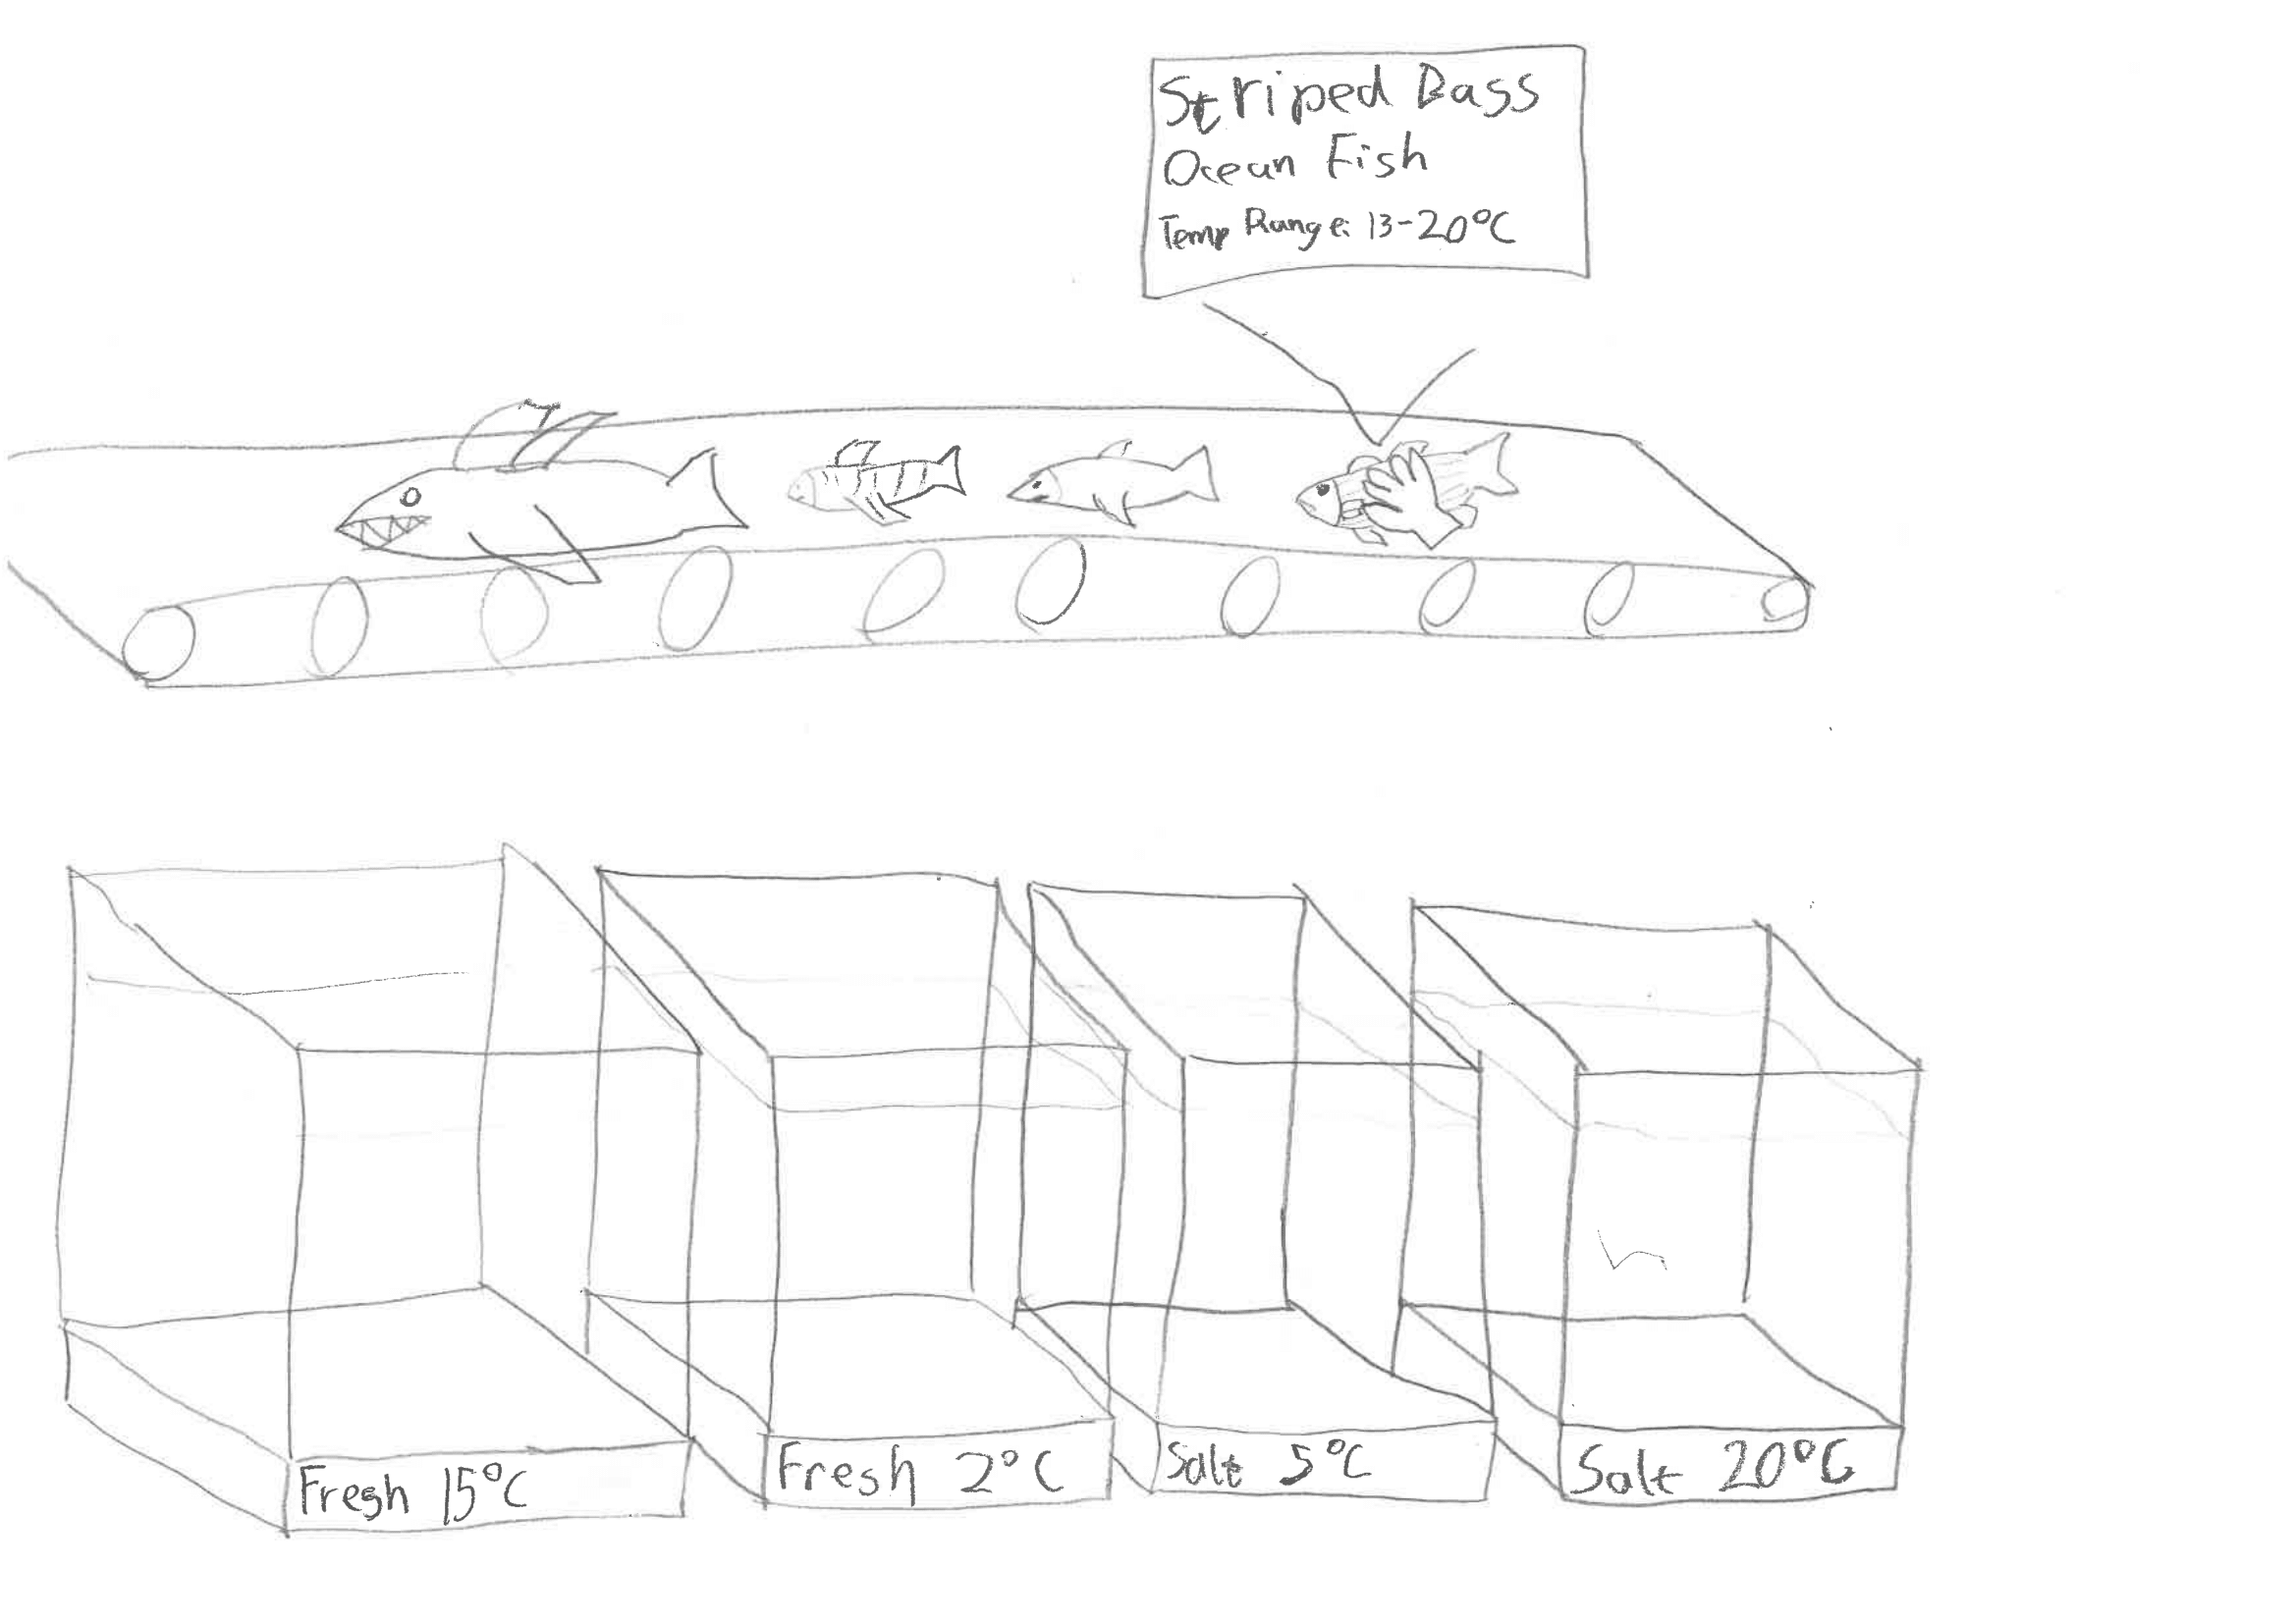
\includegraphics[width=\textwidth]{Sketches/GameConcept2.png}
\caption{General Sketch for the way the game might look}\label{GameConceptSketch2}
\end{figure}
The current idea is for the presentation of each habitat the player can sort fish into to be an aquarium. Each fish is brought out to the player on a conveyor belt, with the length of the belt representing the time limit for the fish, as the fish times out upon reaching the end of it. The players cursor is represented with an open hand, which will visibly grab a fish when the player clicks it. This concept for the game graphics can be seen in Figure \ref{GameConceptSketch2}.\\

An older concept for the game sees the player instead grab fish from a plate and drop them into the waters on a map of a landmass, as some sort of deity taking control. In this concept, the timer for an individual fish would be less clear however, and it would be harder to tell which features the given waters have. It would also be harder to introduce more habitats, which would close that avenue of aggregation. Consequently, this concept has been mostly discarded, although certain ideas from it might be revisited later, and the sketch for this version has been included for posterity in Figure \ref{GameConceptSketch1}.
\begin{figure}
\centering
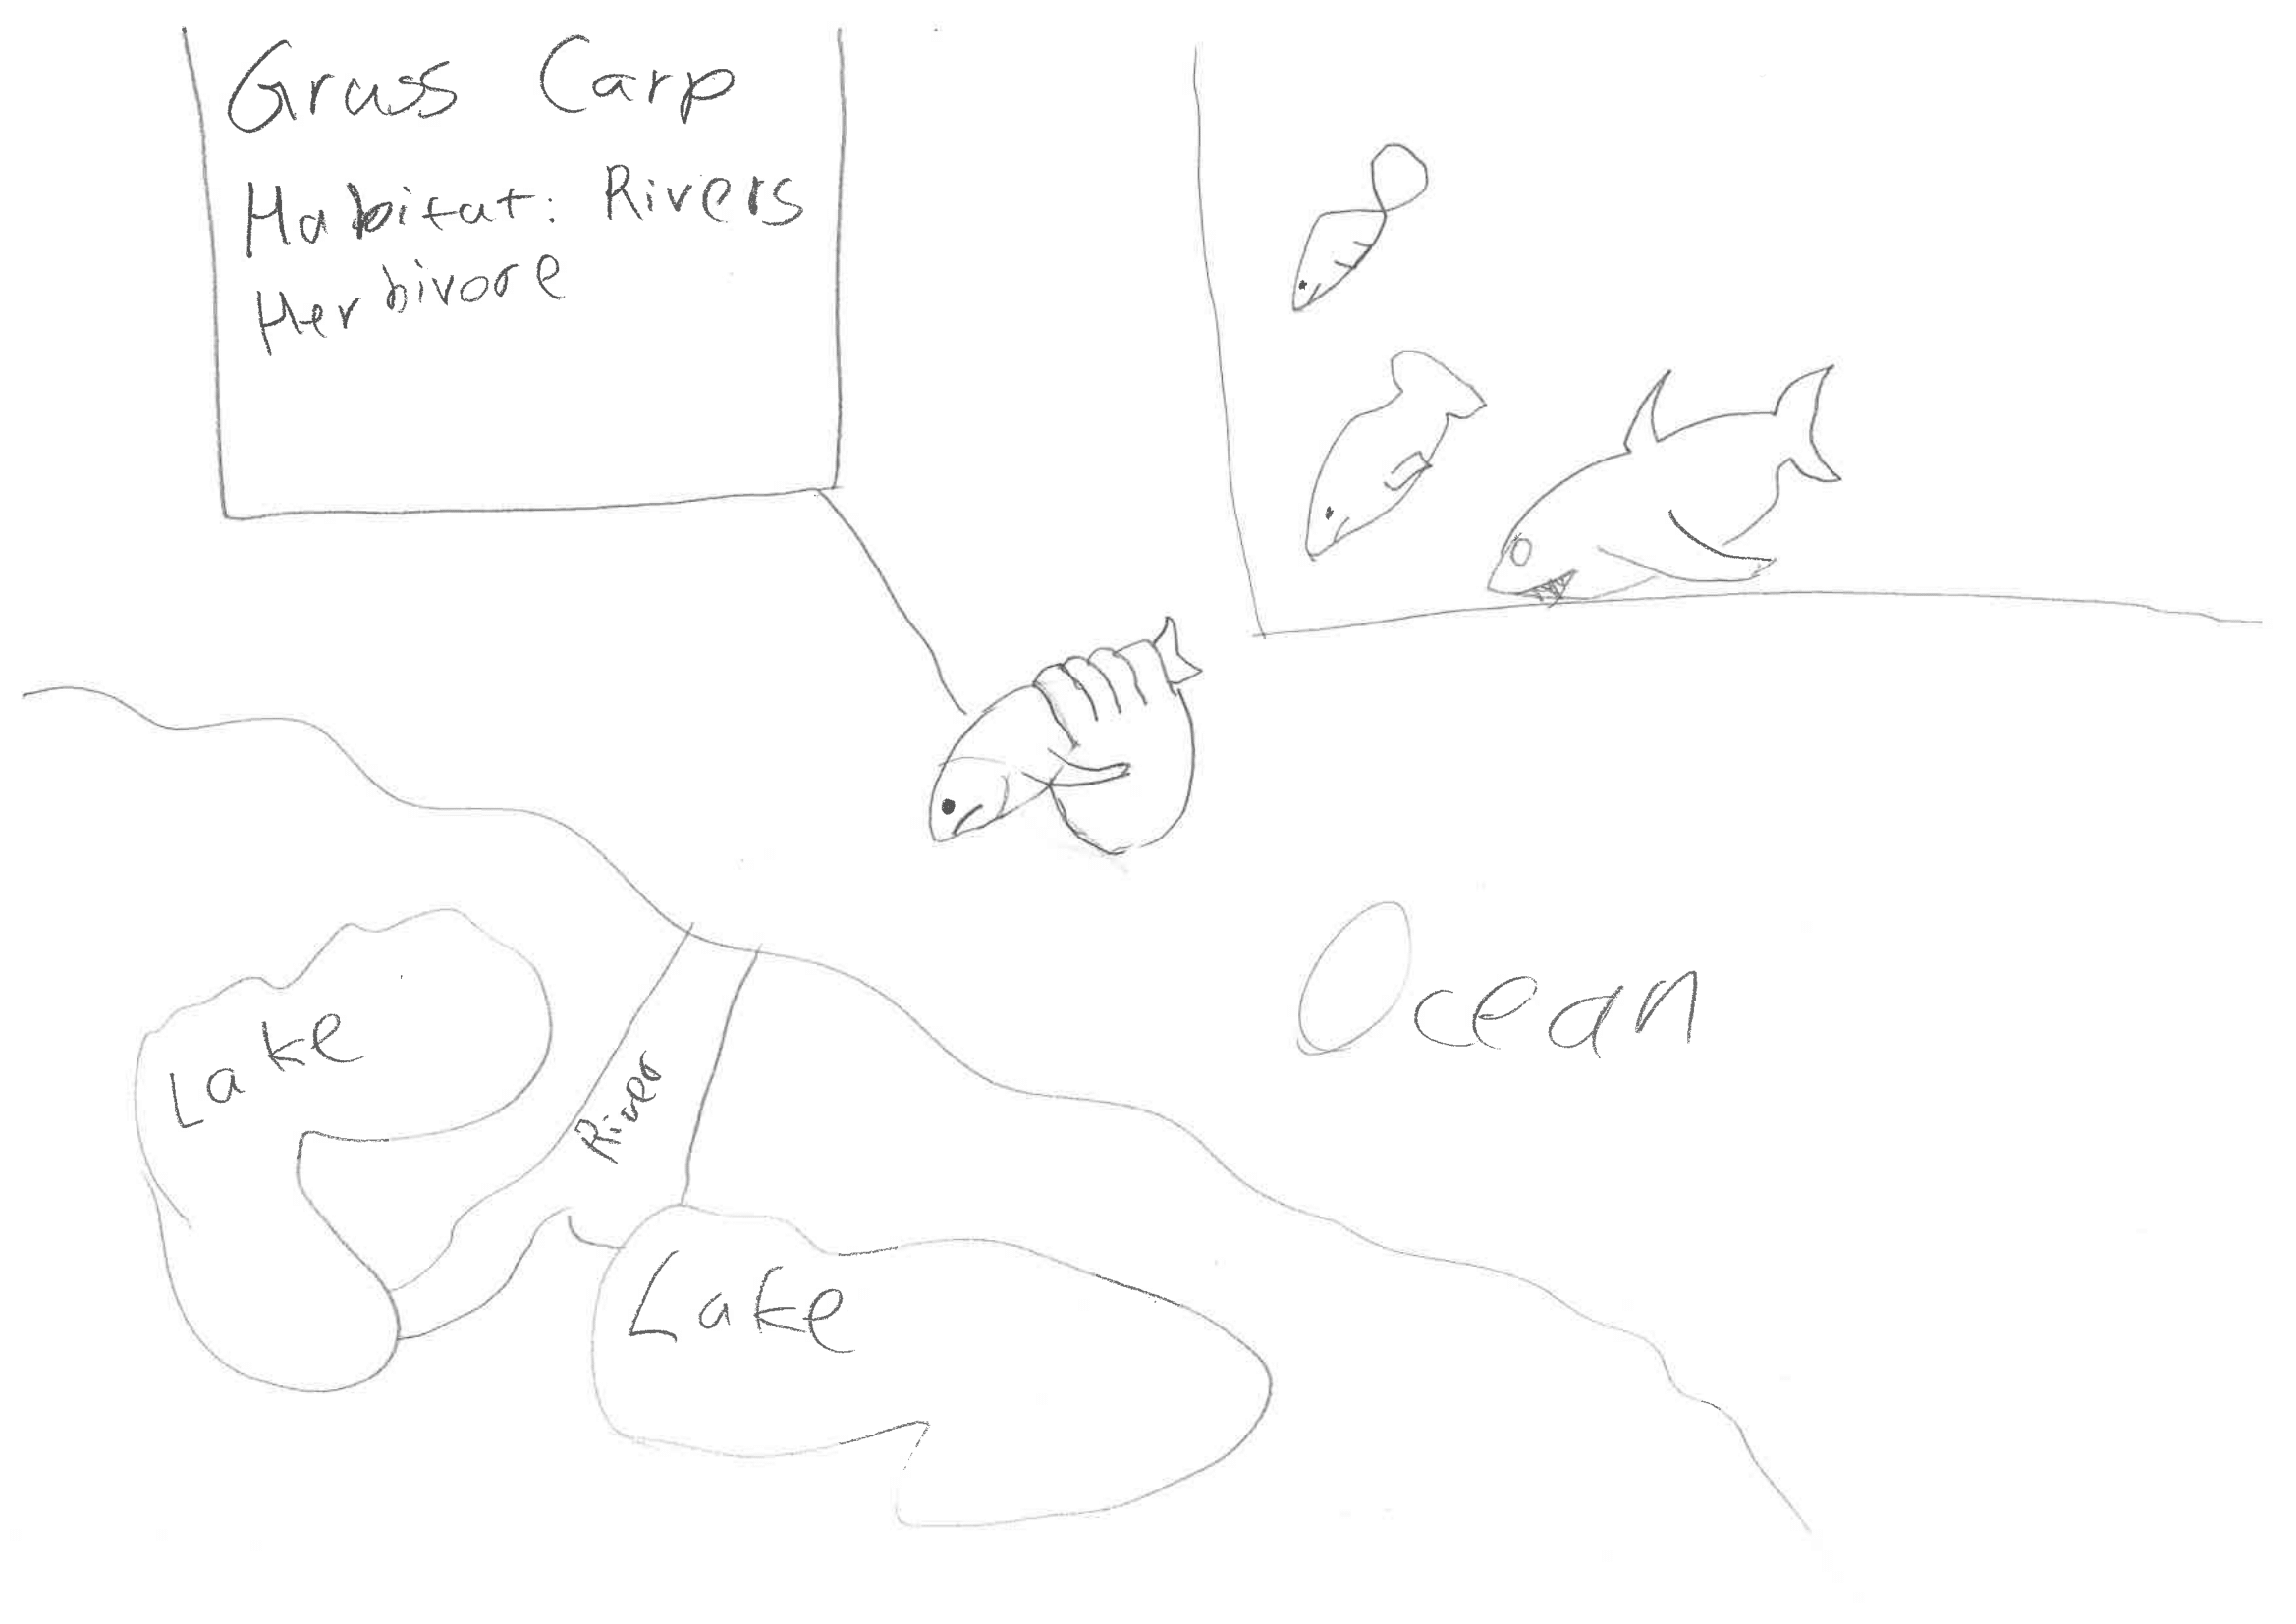
\includegraphics[width=\textwidth]{Sketches/GameConcept1.png}
\caption{Sketch of an older version of the game appearance concept}\label{GameConceptSketch1}
\end{figure}

\subsection{Difficulty Ramping}
The game starts out sending a fish on the conveyor every two or so seconds, with the fish taking 10-15 seconds to reach the end of it. For every five or so points the player scores, the game will likely either slightly speed up the conveyor making fish time out faster, or lessen the time gap between when the fish are sent out. For every ten or so points, a new fish for the player to sort between is sent out, with the starting amount being 2 different species (a freshwater and a saltwater fish).\\

The game starts out with just two aquariums, one being labeled Saltwater and the other Freshwater. At 30 or so points, the amount of aquariums is increased from two to four, with temperature now being a condition. At 100 or so points, a fifth or even sixth aquarium might be added.\\

If the fish start getting introduced with small enough gaps, perhaps a second conveyor would open to prevent them from overlapping.\\

\subsection{Potential further scalability}
Potentially, aquariums might be replaced at certain thresholds, shaking up which habitats the player needs to sort between. Alternatively, more habitat conditions such as water pH, or whether specific fish would eat each other might also be added. In determining the best way to ramp difficulty as the game goes on, the developers might find it prudent to consult an actual marine biologist, as they'd know the important factors of habitat conditions better.
\end{document}